%課題研究レジュメテンプレート ver. 1.2

\documentclass[uplatex]{jsarticle}
\usepackage[top=20mm,bottom=20mm,left=20mm,right=20mm]{geometry}
\usepackage[T1]{fontenc}
\usepackage{txfonts}
\usepackage{wrapfig}
\usepackage[expert,deluxe]{otf}
\usepackage[dvipdfmx,hiresbb]{graphicx}
\usepackage[dvipdfmx]{hyperref}
\usepackage{pxjahyper}
\usepackage{secdot}

\makeatletter
  \renewcommand{\section}{%
    \if@slide\clearpage\fi
    \@startsection{section}{1}{\z@}%
    {\Cvs \@plus.5\Cdp \@minus.2\Cdp}% 前アキ
    {.5\Cvs \@plus.3\Cdp}% 後アキ
    %{\normalfont\Large\headfont\raggedright}}
    {\normalfont\raggedright}}

  \renewcommand{\subsection}{\@startsection{subsection}{2}{\z@}%
    {\Cvs \@plus.5\Cdp \@minus.2\Cdp}% 前アキ
    {.5\Cvs \@plus.3\Cdp}% 後アキ
    %{\normalfont\large\headfont}}
    {\normalfont}}

  \renewcommand{\subsubsection}{\@startsection{subsubsection}{3}{\z@}%
    {\Cvs \@plus.5\Cdp \@minus.2\Cdp}%
    {\z@}%
    %{\normalfont\normalsize\headfont}}
    {\normalfont}}
\makeatother
%ここから上を編集する必要はない.




\title{\vspace{-14mm}ゲームソフトの発売延期とユーザ評価の相関分析}
\author{PMコース 矢吹研究室 1342014 泉 雄太}
\date{}%日付を入れる必要はない.
\pagestyle{empty}%ページ番号は振らない.
\begin{document}
\maketitle





\section{研究の背景}


現代では,消費者がネット上のレビューなどを見て意思決定することは,当たり前のことになりつつある.そのため,様々な製品がレビューの影響を受けている.

特にゲームソフトの売り上げはレビューの影響を強く受けている.ゲーム雑誌には30年近く前からゲームソフトのレビューが載っており,レビューを見る文化が消費者に根付いているからだ.

なので,ゲームソフト開発プロジェクトでは,製品の発売を延期し,品質の向上をはかる戦略が有効である.それはゲームソフトが娯楽であるがゆえに,ユーザが発売延期をある程度許容できることにも起因する.

そこで,発売延期とレビューの間には,相関関係があるのではないかと考えた.もし相関があれば,延期日数が発表された段階でレビューを予測することが可能になる.

\section{研究の目的}

発売延期とレビューの相関関係を調査する.

\section{プロジェクトマネジメントとの関連}

ゲームソフト開発プロジェクトにおける発売延期について新しい認識を得ることができる.

\section{研究の方法}


本研究は2段階に分かれる.
\begin{enumerate}
\item 対象となったゲームソフトに関する情報を調査する.
\item 調査したデータの分析をする.
\end{enumerate}

2003年に発売したプレイステーション2用ゲームソフトを対象として以下の7項目を調査する.

\begin{enumerate}
\item 発売日
\item 販売元
\item レビュー
\item ゲームソフトのジャンル
\item 延期回数
\item 延期日数
\item ゲームソフトの正式タイトル
\end{enumerate}

レビューとゲームソフトジャンルの調査には,ユーザーレビューを行っている「PS2ゲームソフトどうなの?」というWebサイトを利用する.本研究ではこのWebサイトにおける「総評」という項目のみをレビューとして扱う.この項目はゲームソフトの総合的な品質を100点満点で評価したものである\cite{review}.

発売延期に関する調査は,週刊ファミ通の後述のWikipediaのページの情報と,「新作ゲームソフト発売スケジュール」の「発売日や価格に変更のあったソフト」欄及び「発売日スケジュール表に初登場した新作ソフト」欄を見比べることで行う\cite{fami}.

ゲームソフトの正式タイトルと販売元と発売日の調査は,Wikipediaの「PlayStation 2のゲームソフトタイトル一覧 (2003年)」というページをXMLファイルとして出力したものをもとに行う\cite{wiki}.

各情報に誤りがあると感じられた場合は,対象となるゲームソフトの公式ホームページ,またはソニーコンピューターエンタテイメントの提供するプレイステーション公式サイトにて確認する.

データの分析は以下のことを行う.

\begin{enumerate}
\item 相関分析により,延期日数とレビューの相関係数を求める.
\item 相関分析により,延期回数とレビューの相関係数を求める.
\item レビューを縦軸,延期日数を横軸とした散布図を作成する.
\end{enumerate}


\section{現在の進捗状況}

\begin{wrapfigure}[14]{r}{9cm}
\vspace*{-\intextsep}
%\includegraphics[width=図の幅,clip]{ファイル名}\label{参照用ラベル}
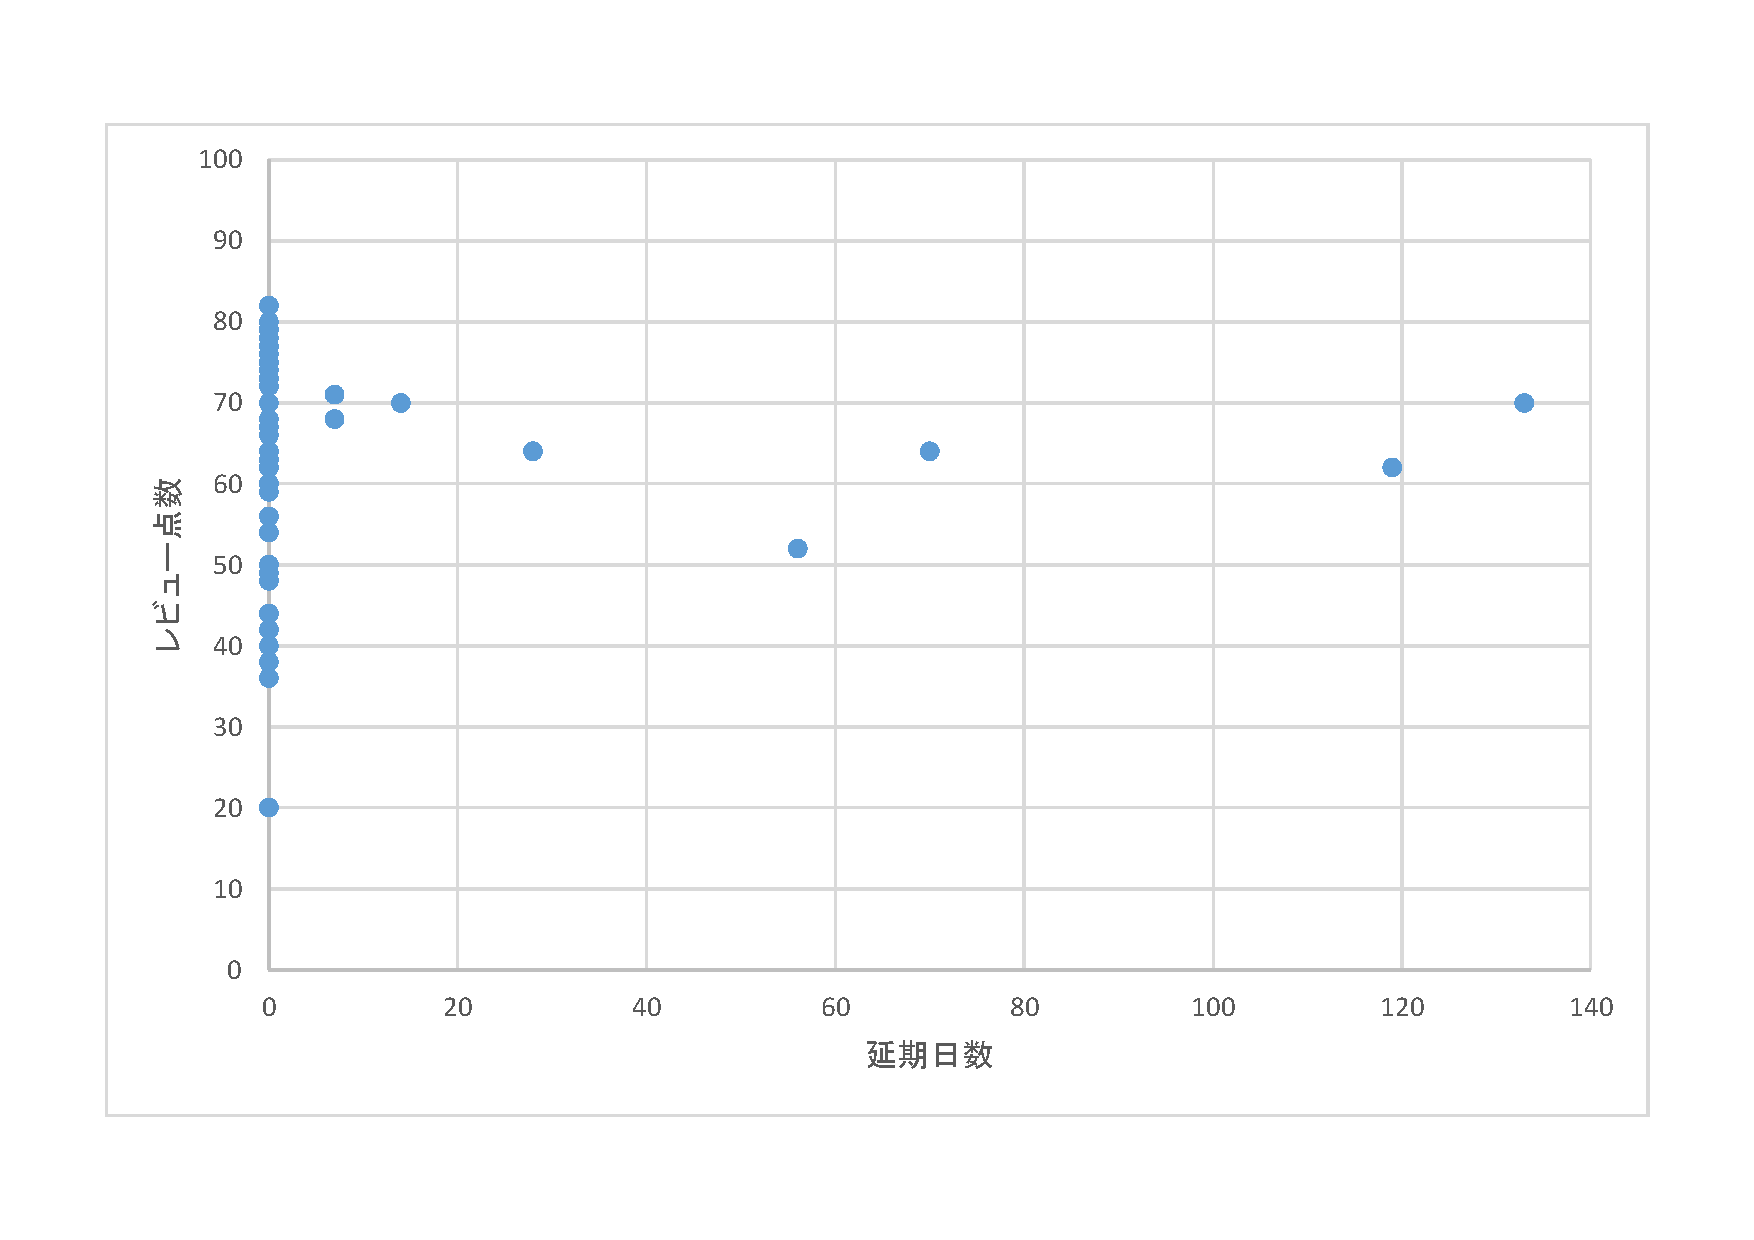
\includegraphics[width=9cm,clip]{sanpu.pdf}
\caption{延期日数とレビューの散布図}\label{散布図}
\end{wrapfigure}

2003年発売のプレイステーション2用ソフトのうち,6月と7月に発売が発表されたことのあるゲームソフト71本を対象に調査を行い,その結果をもとに散布図の作成と相関分析を行った.
ただし,対象となったゲームソフトのうち11本はレビューが存在しなかったため,使用したデータは60件となった.また,延期したゲームソフトは60本中8本だった.

レビューの点数と延期回数の相関係数は-0.002という値になった.レビューの点数と延期日数の相関係数は-0.007という値になった.両方とも負の相関係数となっているが,値が非常に小さく相関があるとは言えない.

図1はレビューの点数を縦軸,延期日数を横軸とした場合の散布図だ.発売延期をしたゲームソフトのレビューが,全体に対して特別大きかったり小さかったりする特徴は見当たらない.

\section{今後の計画}


現状,データ数がかなり少なく,延期したゲームソフトが8本しかなかったため,十分な分析ができていないといえる.

また,調査対象がプレステーション2用ソフトだけなので,データに偏りがあるといえる.

上記2つの点を踏まえ,以下を今後の計画とする.

\begin{enumerate}
\item 調査対象とするゲームソフトに,PS3用ソフト,ゲームキューブ用ソフト,Wii用ソフトを追加する.
\item 調査対象に追加した各ハードごとに100件以上のデータを集める.また,PS2用ソフトのデータも追加で50件集める.
\item 論文の執筆を行う.
\end{enumerate}

\bibliographystyle{junsrt}
\bibliography{biblio}%「biblio.bib」というファイルが必要.

\end{document}



